


\subsection{Model setup}
% CEDRIC: I cant figure out a nice order and structure for this section, as all sections seem to be intertwined, for me it seems logic to start with parameter testing, but those are done using on the "south flank" setup from flank simulations and the values for Mount Etna, so I do not know. I've left them as seperate blocks, could you have a look with your more experienced view in paper writing what should be a clear / proper structure here% 

\subsubsection{Synthetic topography: Flank simulations}
Given that the majority of lava flows are located on the flanks of volcanoes, simulating volcanic flanks is a relevant and intuitive starting point for our initial generic modeling setup. While the magnetization direction remains consistent, the dip direction of the surfaces on these flanks varies. To explore the impact of these variances, we established a model setup dedicated to flank simulations, as illustrated in Figure \ref{fig:flanksim}. In our approach, the flank topography is emulated using a sine approximation on a slope, with the sine function capturing the characteristic ridges and gullies of volcanic topography.

In these simulations, a wide range of parameters can be adjusted to investigate their influence on the magnetic field. These include the surface slope, the amplitude and wavelength of the sine function, and the angle between the sine wave's direction and either the x-axis or y-axis—depending on the flank, as depicted in Figure \ref{fig:bdeg}.

For alignment with our case study, parameter estimates aiming to replicate the ridges and gullies of Mount Etna were derived from aerial images and Digital Elevation Models (DEMs). The estimated amplitude, wavelength, and angle for the slope were 8m, 25m, and 6 \degree, respectively. 

Flank simulations were done using a domain of 250x250x20m with 375x375x10 elements (per predetermined required parameters), with computation done a path of 47 points located one meter above the center of the domain. The sine wave was shifted to create the exact same topography underneath the path at the center of each flanks.

\subsubsection{Mount Etna}
To compare to the field measurements in this study, the uniform remnant magnetization intensity assigned to the matter was: 7.5 A/m. This value compares well with both the TRM found in samples taken from the lava flows in the field \parencite{Meyer23} and with previous paleomagnetic studies of Etnean lavas \parencite{Nicolosi14}; a bulk magnetization intensity of 8 A/m was measured, with values ranging between 5 and 13 A/m. However, both much lower and higher values have also been reported in other studies, 0.1-1 A/m and 20 A/m by \parencite{Tanguy04, Speranza06}, respectively. Clearly displaying the large dispersion of the measurements or values of the magnetization in Etnean lavas. The inclination of the magnetization used in this study is \ang{57}. This value was computed from Mount Etna's average latitude using the Geocentric Axial Dipole hypothesis, ($\tan{I} = 2\tan({lat})$). The declination was assumed to be \ang{0} (parallel to the present geomagnetic field) and from this the components of the magnetization were calculated. 

\subsubsection{Parameters of the domain}
Certain limitations exist in reproducing any shape with a discretized domain and can lead to errors in computed values. To be able to compute accurate anomalies above topographies certain parameters of the domain need to be determined first; the minimum amount of elements to accurately represent volcanic terrain and the minimum size of the domain to limit the edge effect. This effect at the edges of the simulated domain results from the cutoff, the edge, producing its own (magnetic) anomaly. Our objective is to limit the edge effect, whilst also constraining the absolute size and resolution of the domain to keep computation time and effort as low as possible. These parameters were determined using a domain with a synthetic topography, as using a DEM limits certain parameters. 
The test will start at a high resolution, while continuously decreasing the amount of elements we expect to find a threshold at which decreasing the amount further would result in erroneous values. \\  We will therefore continually increase the size of the domain until the computed magnitude of the magnetic field at a point above the center of the domain is constant. \\ Upon doing so in depth, a problem arises; the exact nature of the magnetization in the underlying flows and deeper is unknown, but a constant magnetization is still assumed. The assumption of constant magnetization now expands deeper, eventually stretching to the full pile of volcanic flows of the Etna. To validate this assumption we refer to the geomagnetic history of Mount Etna. The last reversal of Earth's magnetic field was dated around $\sim795$ ka ago \parencite{Singer19} and the first volcanic activity of Mount Etna was dated around $\sim500$ ka ago \parencite{Branca08}. So no reversals are expected to be present in the pile, so, the depth can be increased up to the required limitation of any edge effect. Considering the amount of elements in depth, it is expected that changing this has no influence on the results. Again, as all internal forces should cancel, increasing this number should only result in a longer computation time.
\\ One last issue to contemplate, is the shape of the bottom of the mesh. As mentioned before, these can be simulated in two ways: (1) use the same topography as the top surface, (2) produce a flat bottom. As our computational solution is a surface integral and the interior contributions should cancel out, we can understand the possible repercussion of this predicament. Neither is an accurate representation of reality and from theory we know the effect could be significant. Therefore, the differences need to be investigated and both methods will be used and compared.  


\par The tests were done on a plane with an elevation 1 m above the surface, the height of lowest path for most sites. As the lowest elevation requires the largest resolutions and domain size, this setup will define the threshold. The test were done using the south flank setup as described in the flank simulations. It is uncertain if the parameters determined by these test translate directly to the required threshold when computing above the DEM.  The real topography on Mount Etna is likely to include more complex and larger structures. A larger structure to introduce a larger anomaly that could therefore carry further; as the strength of a magnetic anomaly produced by an object is proportionally related to its size (volume or weight) and restrained by the distance \parencite{GRIFFITHS}.  Therefore, these parameters need to be revisited in future DEM tests. \\
\begin{figure}
\centering
   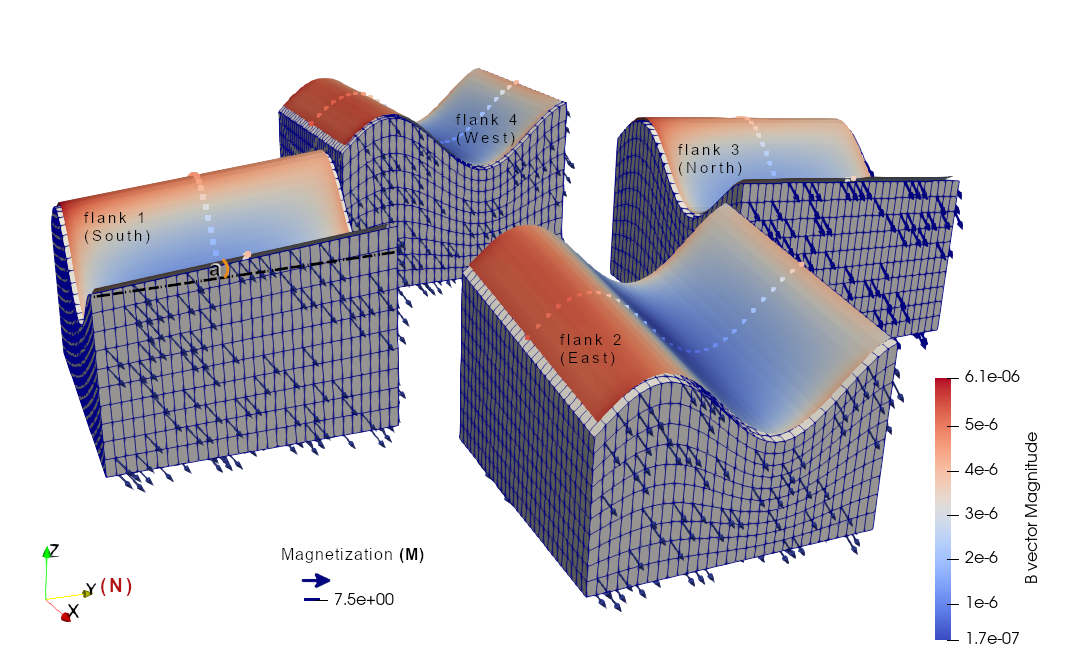
\includegraphics[width=0.5\textwidth]{Afbeeldingen/flanksim/flanks2edit.png}
    \caption{Flank simulation on the Etna. ($\mathbf{M}$) = 7.5 $A/m$ (arrows). The slope ($a$ in Figure, $sf$ in code) is 0.15. The computations of the magnetic field ($\mathbf{B}$) above the flanks are done on a plane and path. The flanks are numbered as displayed. For visual display the size of the domain here is much smaller than in the test.}
    \label{fig:flanksim}
\end{figure}
\begin{figure}
\centering
   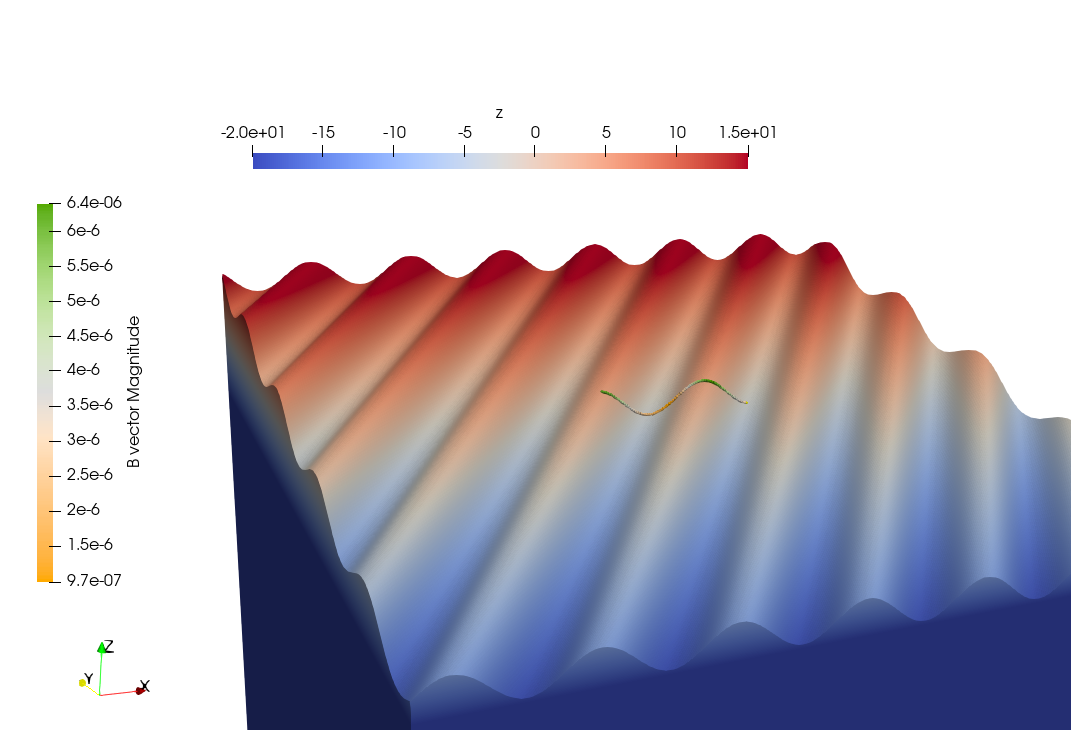
\includegraphics[width=8cm]{Afbeeldingen/methods/bdegflank.png}
    \caption{$bdeg$ is \ang{-31}, an example of a variation possible while doing flank simulations tests.}
    \label{fig:bdeg}
\end{figure}
\begin{figure}
\centering
   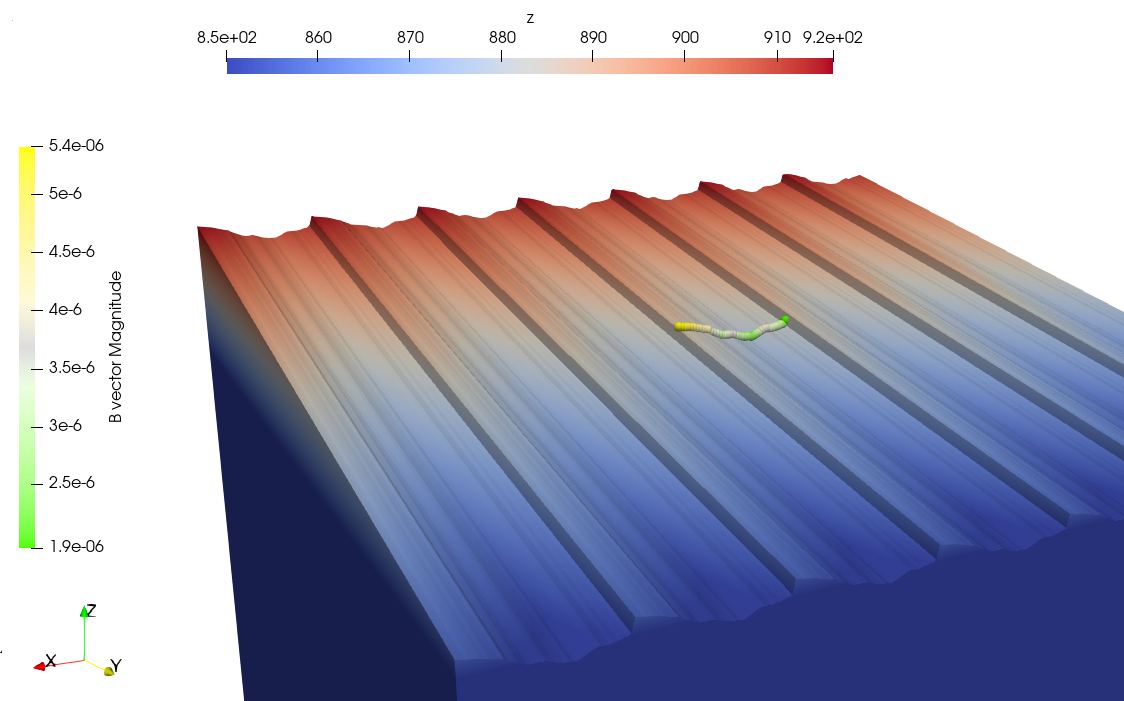
\includegraphics[width=8cm]{Afbeeldingen/flanksim/s3_p1_pathdem3.png}
    \caption{A topography based on field path of site 3, path 1, iterated 7 times, on the North flank of Mt. Etna. The surface is placed on a slope with $sf$=0.15 dipping north.}
    \label{fig:dempath}
\end{figure}

\subsubsection{Topography from Digital Elevation Models at field paths}
The 2x2m spatial resolution DEM \cite{ATA} is geo-referenced using the ROMA 40/EST - EPSG 3004 in Gauss–Boaga projection. We converted the 2m DEM to WGS84 UTM 33N in ArcGIS Pro using bilinear interpolation. This 2m DEM is publicly accessible through the web-sphere of SITR. While detailed information regarding data acquisition methods is absent, it is understood that the original data source was LiDAR. In contrast, the 5x5m spatial resolution DEM presented in \cite{Bisson16} is geo-referenced using the WGS84 UTM 33N System, boasting a vertical accuracy with a root-mean-square-error of $\pm 0.24 m$. This DEM is derived from data obtained using airborne LiDAR. Regarding the 5m DEM, it is stated that the DEM was obtained by resampling of an original 2m DEM using the nearest neighbors algorithm \parencite{Bisson16}. Subsequently, they conclude that the vertical and horizontal accuracy of the original data is conserved. Both DEMs were cut to different sizes, ranging in spatial extent from 50x50 m to $\sim$2x2km around the sites. While retaining the original 2m accuracy is commendable, working with a 5m DEM inherently restricts us to a 5m resolution, hence capping our potential accuracy. Despite multiple attempts, the original 2m DEM remained elusive, compelling this study to proceed with the 5m DEM.\par 
\par
To reproduce the field data, a path can be generated based on the GPS coordinates of field data by using the x \& y coordinates from the field path, the height is computed at a constant value above the surface of the DEM. The GPS field data in this study was converted from decimal degrees to the WGS84 UTM 33N system to match the DEMs. The DEM cut's corner x- and y-coordinates were subtracted from the field coordinates, ensuring alignment. The height of the GPS placement on the measuring device, 2m above the surface \parencite{deGroot19}, was subtracted from the field data beforehand. 
\par
Two different reference fields were added to the computed values: The IGRF at the site or the average on the Etna at the moment of measuring (April 2018) and $\mathbf{B_{ref}}$. The latter is the computed mean of all field data from all paths at one site. Inputting the appropriate site (and path) details triggers an automatic retrieval of the relevant DEM, reference field, IGRF, magnetization, etc.

